% STAR: Stability-aware learned next-hop selection for TRCN.
% Compile:  latexmk -xelatex main.tex      (biber runs automatically)
% Switch "jou" to "man" for an APA 7 manuscript-format submission.
\documentclass[jou,a4paper,11pt,floatsintext]{apa7}
\usepackage[american]{babel}
\usepackage{csquotes}
\usepackage[style=apa,backend=biber]{biblatex}
\addbibresource{../references.bib}
\usepackage{fontspec}
\usepackage{xeCJK}
\setCJKmainfont[AutoFakeSlant=0.15]{Heiti TC}
\usepackage{amsmath,amssymb,mathtools}
\usepackage{booktabs,tabularx,multirow}
\usepackage{graphicx}
\usepackage{xcolor}
\usepackage{algorithm}
\usepackage[noend]{algpseudocode}
\usepackage{tikz}
\usetikzlibrary{arrows.meta,positioning,calc}
\hypersetup{hidelinks}
\newcolumntype{Y}{>{\raggedright\arraybackslash}X}
\DeclareMathOperator*{\argmax}{arg\,max}
\DeclareMathOperator*{\argmin}{arg\,min}
% Headline numbers (from results/headline.json, evaluation seeds 100-119).
\newcommand{\STARmainPDR}{97.7\%}
\newcommand{\STARmainSOS}{100\%}
\newcommand{\ETXmainPDR}{89.6\%}
\newcommand{\PROmainPDR}{90.5\%}
\newcommand{\STARafterPDR}{92.8\%}
\newcommand{\ETXafterPDR}{82.5\%}
\newcommand{\PROafterPDR}{84.9\%}


\title{Learning Which Route to Trust: Stability-Aware Bayesian Next-Hop Selection for Infrastructure-Independent Disaster Messaging}
\shorttitle{Stability-Aware Learned Routing}
\leftheader{Stability-Aware Learned Routing}
\authorsnames{Pinyen Cheng}
\authorsaffiliations{{Taoyuan, Taiwan}}

\abstract{When cellular sites lose power and backhaul after a disaster, short text messages must hop between phones, shelters, and regional gateways over intermittent, low-rate links. Choosing the next hop is then a prediction problem: which neighbor is most likely to deliver the message before it expires? We present STAR (Stability-aware TAR routing), a fully local next-hop policy for the Taiwan Resilient Communication Network that (a) predicts route stability $\Psi$, the probability of on-time delivery, from discounted Bayesian posteriors over link frame success and availability combined with loop-free, authenticated distance-vector advertisements; (b) decides with a priority-aware rule that is risk-averse and replicates distress messages, yet explores with Thompson sampling on non-urgent traffic; and (c) learns from outcomes through fragment acknowledgments, signed end-to-end receipts treated as falsifiable deadlines, and overheard forwarding, which together calibrate trust in each neighbor's route claims. In a discrete-event simulator with LoRa time-on-air and airtime-accounted control traffic, evaluated on 20 held-out seeds of a synthetic two-region disaster network, STAR delivered \STARmainPDR\ of messages and all distress messages, against \ETXmainPDR\ for a loop-free ETX distance-vector baseline and \PROmainPDR\ for PRoPHET, with 44\% lower median latency than the former. After a simulated aftershock it delivered \STARafterPDR\ versus \ETXafterPDR\ and \PROafterPDR. Under route poisoning it retained several times the delivery of an unprotected distance-vector protocol, although replication-based protocols remained more robust. Gains vanish at saturation. All results are synthetic.}
\keywords{delay-tolerant networking, learned routing, Thompson sampling, Bayesian link estimation, disaster communication, LoRa, route poisoning}
\authornote{
  Simulation code, raw results, and scripts that regenerate every table and figure are available at \url{https://github.com/chengmatt416/trcn}. This work has no affiliation with any government agency; no radio was operated and no personal data were collected. The author used generative AI assistance in this work (see the Use of Generative AI section). Correspondence concerning this article should be addressed to Pinyen Cheng, Taoyuan, Taiwan.
}

\begin{document}
\maketitle

\section{Introduction}

A disaster that cuts grid power silences cellular sites long before it damages them. After the magnitude 7.2 earthquake off Hualien on 3 April 2024, Taiwan's three major carriers reported 172 affected base stations, mostly because of interrupted power and transmission links \parencite{cna2024}, and a highway collapse left the Tianxiang area without communication until satellite terminals were airlifted in three days later \parencite{moda2024}. Backhaul can be restored at a few points; what remains missing is a path between \emph{people, shelters, and coordinators} in the last few kilometers.

The Taiwan Resilient Communication Network (TRCN) is a research architecture for that gap: phones reach shelters over Wi-Fi Aware or Bluetooth, shelters and regional gateways form a LoRa mesh, and regions interconnect over whatever backbone survives. Messages are short, end-to-end encrypted, and carried store-and-forward with per-hop custody and recipient-signed receipts. The earlier TRCN prototype routed with \emph{preloaded} next hops and ignored control-plane airtime, which its own documentation lists as the first limitation to fix.

This paper addresses that limitation. Its research question is: \emph{Using only information a node can observe locally, can a node predict which neighbor offers the most stable route to a destination, act on that prediction, and improve it from the outcomes of its own decisions?} Stability here has a precise meaning: the probability that a message is delivered before its deadline.

Two properties make the problem hard. First, links in a disaster are \emph{intermittent and non-stationary}: a Wi-Fi link to a phone appears and disappears as people move or screens sleep; a LoRa link fades with interference; an aftershock removes links permanently. Classic shortest-path metrics such as ETX \parencite{decouto2003} capture loss but not availability or deadlines; DTN utilities such as PRoPHET \parencite{lindgren2003} capture encounter history but replicate aggressively, which LoRa's scarce airtime cannot afford \parencite{bor2016}. Second, feedback is \emph{delayed and partial}: a node sees per-hop acknowledgments quickly, but whether a message reached its destination is known only to the source and only when a receipt returns, if it returns at all.

\textbf{Contributions.} (1) We formulate next-hop selection in TRCN as on-line prediction of a deadline-aware stability score $\Psi$ and derive a tractable, fully local estimator that composes Bayesian link posteriors with loop-free, authenticated distance-vector summaries (see \nameref{sec:model}). (2) We give a priority-aware decision rule: risk-averse with bounded replication for distress traffic, Thompson-sampling exploration for non-urgent traffic, and explicit hold decisions for store-carry-forward (Algorithm~\ref{alg:decide}). (3) We close the learning loop with three outcome channels (selective fragment acknowledgments, receipts treated as falsifiable delivery deadlines, and watchdog overhearing) and show that \emph{trust as calibration} of neighbors' claims bounds route poisoning. (4) We release an open simulator with LoRa time-on-air, airtime-accounted control traffic, collisions, crashes, and blackhole attacks, and evaluate STAR against six baselines over 1{,}520 runs with held-out seeds (see \nameref{sec:method} through \nameref{sec:results}).

\section{Related Work}

\textbf{Delay-tolerant routing.} DTN routing \parencite{fall2003,jain2004} spans replication (epidemic routing, spray-and-wait), utility-based forwarding (PRoPHET, MaxProp), resource-allocation formulations (RAPID), and contact-plan routing for scheduled links \parencite{vahdat2000,spyropoulos2005,lindgren2003,burgess2006,balasubramanian2007,fraire2021}. Replication buys robustness with airtime and buffer space; contact-plan routing assumes a known schedule, which disasters do not provide. Simulation tools such as the ONE \parencite{keranen2009} popularized evaluation under mobility traces. TRCN's shelter backbone is mostly static but intermittent, which places it between classic mesh routing and opportunistic DTN.

\textbf{Link-quality-aware mesh routing.} ETX and its time-based variants weight links by expected transmissions \parencite{decouto2003}; link estimators are surveyed by \textcite{baccour2012}, and burst-error channels go back to the Gilbert model \parencite{gilbert1960}. Distance-vector protocols avoid loops with destination sequence numbers \parencite{perkins1994}; Babel adds a feasibility condition that keeps routing loop-free even during convergence \parencite{rfc8966}. STAR inherits Babel's feasibility condition but replaces its additive metric with a probabilistic, deadline-aware score.

\textbf{Learning-based routing.} Q-routing learns per-destination delivery-time estimates from neighbor feedback \parencite{boyan1994} and has predictive and dual variants \parencite{choi1996,kumar1997}. Reinforcement learning has been applied to DTN forwarding and replication \parencite{rolla2013,dudukovich2017}; \textcite{bhavani2023} review machine-learning DTN routing, and graph neural networks model network performance in software-defined networks \parencite{rusek2020}. Bandit formulations of routing study regret when per-link or end-to-end feedback is observed \parencite{gai2012,talebi2018}; a key finding is that per-link feedback is far more valuable than end-to-end feedback, which motivates STAR's use of fragment-level acknowledgments. Thompson sampling \parencite{thompson1933,russo2018} and its discounted, non-stationary variants \parencite{raj2017,garivier2011,lattimore2020} underlie STAR's exploration and forgetting. Unlike Q-routing, STAR predicts a \emph{probability} of on-time delivery rather than an expected time, and it uses the uncertainty of its own estimates to set exploration and risk by priority.

\textbf{Secure routing.} Secure AODV authenticates sequence numbers with hash chains \parencite{zapata2002}; watchdogs detect neighbors that do not forward \parencite{marti2000}. STAR combines both with outcome-based calibration so that an insider that advertises impossible routes loses traffic quickly.

\textbf{Disaster LoRa networks.} LoRa's range comes with long time-on-air and limited scalability \parencite{augustin2016,bor2016,adelantado2017}. Community stacks such as Meshtastic and Reticulum \parencite{meshtastic,reticulum} and recent field studies \parencite{khamaisi2025} demonstrate off-grid messaging; surveys catalogue the routing challenges of disaster ad hoc networks \parencite{reina2015}. To our knowledge, none of these combines deadline-aware stability prediction, outcome-calibrated trust, and accounted control airtime.

\section{System Model}
\label{sec:system}

\textbf{Network.} Nodes are phones, shelters, regional gateways, coordinators, and relays. A link $\ell=(i,j)$ uses a medium (Wi-Fi Aware, BLE, LoRa with spreading factor $\mathrm{SF}$, Ethernet, or microwave) with a maximum frame size and a per-frame airtime $t_f(\ell)$. LoRa time-on-air follows the Semtech modem equation \parencite{semtech2013}:
\begin{equation}
\begin{split}
t_f = \frac{2^{\mathrm{SF}}}{B}\Big[&(n_{\mathrm{pre}}+4.25) + 8\\
&+ \max\Big(\Big\lceil\tfrac{8L-4\mathrm{SF}+44-20H}{4(\mathrm{SF}-2D_E)}\Big\rceil(c_r+4),\,0\Big)\Big],
\end{split}
\label{eq:toa}
\end{equation}
for payload $L$ bytes, bandwidth $B$, coding rate $4/(4+c_r)$, header flag $H$ and low-data-rate flag $D_E$. LoRa links in a region share one collision domain with probabilistic carrier sense.

\textbf{Link dynamics.} Each link alternates between up and down periods drawn from exponential distributions (a continuous-time on/off process) and, while up, loses each frame independently with probability $q_\ell$. Scenarios may force outages, fail links permanently, or crash nodes, which loses their RAM custody.

\textbf{Messages.} A message $m$ has source, destination mailbox $d$, priority $p\in\{0,1,2,3\}$ (P0 = SOS, P1 = receipts, P2 = private, P3 = supply), wire size (payload plus 192 bytes of envelope and laboratory cryptographic overhead), and a lifetime $T_m$ (900\,s by default). It is fragmented into TDF frames with a 24-byte header. Each hop is an \emph{exchange}: the sender transmits the missing fragments; the receiver returns an acknowledgment carrying a fragment bitmap and, once all fragments have arrived and the message is admitted, a custody decision. Up to four rounds are attempted before the exchange fails and the sender backs off. Custody is not delivery: the source counts a message as delivered only when the destination's signed RECEIPT arrives.

\textbf{Objective and constraints.} Each node $i$ holding a copy of $m$ must decide, using only local state, whether to forward it and to which neighbor $j$, so as to maximize
\begin{equation}
\Pr\big[\text{$m$ delivered before } t_{e}(m)\big],
\end{equation}
with ties broken toward lower latency and higher priority traffic served first. No node has the topology, link states, or other nodes' queues; all control information must be carried in airtime-accounted beacons or acknowledgment piggybacks.

\section{The STAR Model}
\label{sec:model}

\begin{figure*}[t]
\centering
\resizebox{\textwidth}{!}{%
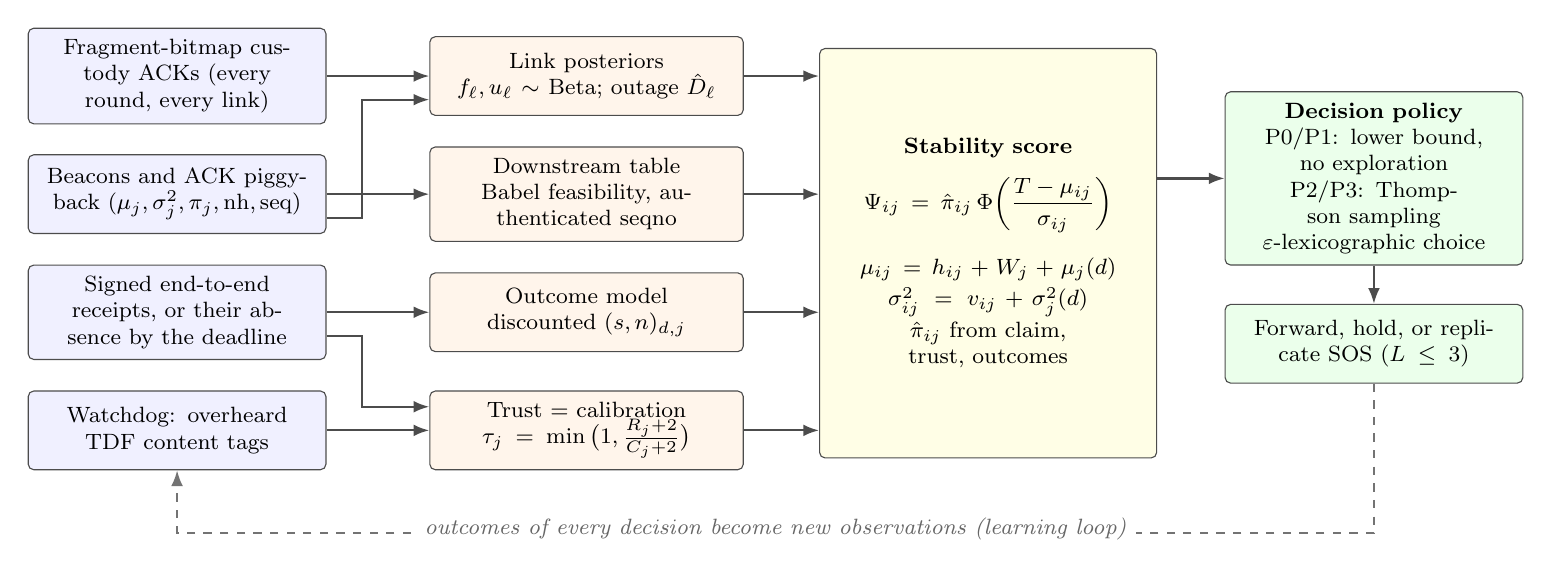
\begin{tikzpicture}[
  font=\footnotesize,
  box/.style={draw=black!70, rounded corners=2pt, align=center, inner sep=4pt, fill=#1},
  box/.default=white,
  obs/.style={box=blue!6, text width=3.5cm, minimum height=1.0cm},
  est/.style={box=orange!8, text width=3.7cm, minimum height=1.0cm},
  dec/.style={box=green!8, text width=3.5cm, minimum height=1.0cm},
  arr/.style={-{Latex[length=2mm]}, thick, black!70},
  fb/.style={-{Latex[length=2mm]}, thick, dashed, black!55}
]
% column 1: observations
\node[obs] (ack)  at (0, 3.6) {Fragment-bitmap custody ACKs (every round, every link)};
\node[obs] (bcn)  at (0, 2.1) {Beacons and ACK piggyback $(\mu_j,\sigma^2_j,\pi_j,\text{nh},\text{seq})$};
\node[obs] (rcp)  at (0, 0.6) {Signed end-to-end receipts, or their absence by the deadline};
\node[obs] (wd)   at (0,-0.9) {Watchdog: overheard TDF content tags};
% column 2: estimators
\node[est] (lp)   at (5.2, 3.6) {Link posteriors\\$f_\ell,u_\ell\sim\mathrm{Beta}$; outage $\hat D_\ell$};
\node[est] (ds)   at (5.2, 2.1) {Downstream table\\Babel feasibility, authenticated seqno};
\node[est] (e2e)  at (5.2, 0.6) {Outcome model\\discounted $(s,n)_{d,j}$};
\node[est] (tr)   at (5.2,-0.9) {Trust = calibration\\$\tau_j=\min\big(1,\frac{R_j+2}{C_j+2}\big)$};
% column 3: score
\node[box=yellow!10, text width=4.0cm, minimum height=5.2cm] (psi) at (10.3, 1.35)
  {\textbf{Stability score}\\[6pt]$\displaystyle\Psi_{ij}=\hat\pi_{ij}\,\Phi\!\left(\frac{T-\mu_{ij}}{\sigma_{ij}}\right)$\\[8pt]$\mu_{ij}=h_{ij}+W_j+\mu_j(d)$\\[2pt]$\sigma^2_{ij}=v_{ij}+\sigma^2_j(d)$\\[2pt]$\hat\pi_{ij}$ from claim, trust, outcomes};
% column 4: decision
\node[dec] (pol) at (15.2, 2.3) {\textbf{Decision policy}\\P0/P1: lower bound, no exploration\\P2/P3: Thompson sampling\\$\varepsilon$-lexicographic choice};
\node[dec] (act) at (15.2, 0.2) {Forward, hold, or replicate SOS ($L\le 3$)};
% arrows
\draw[arr] (ack) -- (lp);
\draw[arr] (bcn) -- (ds);
\draw[arr] (rcp) -- (e2e);
\draw[arr] (wd) -- (tr);
\draw[arr] ([yshift=-3mm]bcn.east) -- ++(0.45,0) |- ([yshift=-3mm]lp.west);
\draw[arr] ([yshift=-3mm]rcp.east) -- ++(0.45,0) |- ([yshift=3mm]tr.west);
\foreach \n in {lp,ds,e2e,tr} { \draw[arr] (\n.east) -- (\n.east -| psi.west); }
\draw[arr] (psi.east |- pol.west) -- (pol.west);
\draw[arr] (pol) -- (act);
\draw[fb] (act.south) -- ++(0,-1.9) -| (wd.south);
\node[font=\footnotesize\itshape, text=black!60, fill=white] at (7.6,-2.15) {outcomes of every decision become new observations (learning loop)};
\end{tikzpicture}}
\caption{The STAR model at one node. Four local evidence streams feed four estimators; their outputs combine into the stability score $\Psi$, which a priority-aware policy turns into a forwarding decision. The outcome of every decision is observed again, closing the learning loop. No component requires global topology knowledge.}
\label{fig:model}
\end{figure*}


Figure~\ref{fig:model} summarizes STAR. Each node keeps four estimators fed by local evidence, combines them into a stability score per neighbor, and applies a priority-dependent decision rule. Table~\ref{tab:params} in the Appendix lists all parameters.

\subsection{Link posteriors}

For each incident link $\ell$, node $i$ keeps two Beta posteriors: frame success $f_\ell\sim\mathrm{Beta}(\alpha_f,\beta_f)$ and availability $u_\ell\sim\mathrm{Beta}(\alpha_u,\beta_u)$. A fragment-bitmap acknowledgment reporting $k$ of $n$ fragments received adds $(k,\,n-k)$ to $(\alpha_f,\beta_f)$. A received beacon, or any acknowledgment, adds one success to $u_\ell$; each missed beacon (detected by a sequence gap) or unacknowledged round adds a failure. To track non-stationarity, before each update every pseudo-count is discounted toward its prior,
\begin{equation}
\alpha \leftarrow \alpha_0 + (\alpha-\alpha_0)\,2^{-\Delta t/H},
\label{eq:decay}
\end{equation}
with half-lives $H_f=900$\,s and $H_u=240$\,s, which is the time-based analogue of discounted Thompson sampling \parencite{raj2017}. Node $i$ also learns the mean outage length $\hat D_\ell$ as an exponentially weighted average of observed silent gaps. Because a long silence is itself evidence, the current availability belief is $\tilde u_\ell = \bar u_\ell\exp\!\big(-(s_\ell-1.6B)^+/\hat D_\ell\big)$, where $s_\ell$ is the time since the last evidence that $\ell$ was up and $B$ is the beacon period.

\subsection{Hop model}

For a message of $n_\ell$ fragments, frame time $t_f$, and acknowledgment time $t_a$, the hop delay has mean and variance
\begin{equation}
\begin{aligned}
h_{ij} &= \frac{n_\ell t_f}{f_\ell} + t_a\big(1+3(1-f_\ell)\big) + (1-\tilde u_\ell)\hat D_\ell + W_i,\\
v_{ij} &= \frac{n_\ell(1-f_\ell)}{f_\ell^2}t_f^2 + (1-\tilde u_\ell)\hat D_\ell^2 + 1,
\end{aligned}
\label{eq:hop}
\end{equation}
where the first terms are the geometric retransmission cost under selective repeat, the third is the expected wait for a down link to return (the exponential-outage assumption makes the residual outage memoryless), and $W_i$ is the node's own high-priority backlog. The value of $f_\ell$ depends on the decision mode: the posterior mean, a lower credible bound $\bar f-1.28\,\mathrm{sd}(f)$, or a Thompson sample.

\subsection{Downstream summaries and loop freedom}

Each node advertises, for a rotating subset of destinations, a compact tuple
\[
\big(\mu_i(d),\,\sigma^2_i(d),\,\pi_i(d),\,\text{next hop},\,\text{seq}_d\big)
\]
in 11 bytes, plus its queue backlog. The same tuple is piggybacked on every custody acknowledgment for the message's destination, so active routes are refreshed at no extra transmission. Loops are prevented with Babel's feasibility condition \parencite{rfc8966}: node $i$ keeps a feasible distance $\mathrm{FD}_i(d)=(s,\mu)$ and accepts neighbor $j$'s route only if $\text{seq}_j>s$, or $\text{seq}_j=s$ and $\mu_j(d)<\mu$; entries whose advertised next hop is $i$ itself are ignored (poisoned reverse). Each destination increments its own sequence number every four beacons, and every number is accompanied, when it changes, by an 8-byte hash-chain authenticator in the style of SAODV \parencite{zapata2002}, so that no relay can advertise freshness the destination has not released.

Given neighbor $j$'s entry of age $a$, with $a^+=\max(0,a-2B)$ the age beyond the expected refresh, the composed route through $j$ has
\begin{equation}
\mu_{ij}=h_{ij}+W_j+\mu_j(d),\qquad \sigma^2_{ij}=v_{ij}+\sigma^2_j(d)+(0.2a^+)^2,
\label{eq:down}
\end{equation}
and a claimed not-lost probability $c_{ij}=\pi_j(d)\,2^{-a^+/H_s}$.

\subsection{Reliability posterior and trust}

Claims are evidence, not facts. Node $i$ keeps, for each neighbor, a trust value equal to the \emph{calibration} of that neighbor's past promises,
\begin{equation}
\tau_j=\min\!\Big(1,\ \frac{R_j+2}{C_j+2}\Big),
\label{eq:trust}
\end{equation}
where $C_j$ accumulates the delivery probability $j$ claimed for each message handed to it and $R_j$ the deliveries actually observed (see \nameref{sec:learning}). For each $(d,j)$ the source also keeps discounted counts $(s_{dj},n_{dj})$ of end-to-end outcomes. The not-lost probability is the posterior mean
\begin{equation}
\hat\pi_{ij}=\frac{K\tau_jc_{ij}+s_{dj}}{K+n_{dj}},
\label{eq:pi}
\end{equation}
with $K=4$ pseudo-observations for the calibrated claim. Neighbors with $\tau_j<0.4$ are excluded; on exclusion, every route and feasible distance learned through $j$ is discarded so that poisoned sequence state cannot starve honest routes.

\subsection{Stability score}

Approximating the remaining delay as Gaussian with mean $\mu_{ij}$ and variance $\sigma^2_{ij}$, a sum of many independent hop components, the predicted probability that a message with remaining lifetime $T$ is delivered on time through $j$ is
\begin{equation}
\Psi_{ij}=\hat\pi_{ij}\;\Phi\!\left(\frac{T-\mu_{ij}}{\sigma_{ij}}\right),
\label{eq:psi}
\end{equation}
where $\Phi$ is the standard normal distribution function. $\Psi$ couples the three ingredients that shortest-path metrics separate: how often a route loses messages ($\hat\pi$), how long it takes ($\mu$), and how predictable it is ($\sigma$). For a message close to expiry, a fast but erratic route can lose to a slower, steadier one; for a fresh message the difference vanishes and delay decides.

\subsection{Decision policy}

\begin{algorithm}[t]
\caption{STAR next-hop decision at node $i$ for a message copy $m$}
\label{alg:decide}
\begin{algorithmic}[1]
\Require copy $m$ (destination $d$, priority $p$, expiry $t_e$, path memory $\mathcal{P}$, tokens $L_m$)
\State $T \gets t_e - t_{\text{now}}$; \textbf{if} $T\le 0$ \textbf{then return} \textsc{Drop}
\State mode $\gets$ \textsc{Sample} if $p\ge 2$ else \textsc{LowerBound}
\ForAll{neighbours $j\notin\mathcal{P}$ with a feasible, authenticated route to $d$ and $\tau_j\ge\tau_{\min}$}
  \State draw or bound $f_\ell$, $u_\ell$ according to mode; compute $(h_{ij},v_{ij})$ \Comment{Eq.~\ref{eq:hop}}
  \State $\mu_{ij},\sigma^2_{ij},\hat\pi_{ij}$ from downstream table and outcome model \Comment{Eqs.~\ref{eq:down}--\ref{eq:pi}}
  \State $\Psi_{ij}\gets\hat\pi_{ij}\,\Phi\big((T-\mu_{ij})/\sigma_{ij}\big)$
\EndFor
\State $\mathcal{C}\gets\{j:\Psi_{ij}\ge\max_k\Psi_{ik}-\varepsilon_p\}$; \ $j^\star\gets\arg\min_{j\in\mathcal{C}}\mu_{ij}$
\If{$\tilde u_{\ell(j^\star)}<0.3$ and no alternative within $\Psi_{ij^\star}/2$ is believed up}
  \State \Return \textsc{Hold} \Comment{store-carry-forward}
\EndIf
\If{$p=0$, $i$ is the source and $\Psi_{ij^\star}<\Psi^\ast$}
  \State $L_m\gets\min\!\big(L_{\max},\lceil\ln(1-\Psi^\ast)/\ln(1-\Psi_{ij^\star})\rceil\big)$ \Comment{SOS replication}
\EndIf
\State \Return \textsc{Forward}$(j^\star,\ \max(1,\lfloor L_m/2\rfloor))$
\end{algorithmic}
\end{algorithm}


Algorithm~\ref{alg:decide} turns scores into actions. \textbf{Risk by priority.} Distress messages and receipts (P0, P1) are scored with lower credible bounds and are never used to explore; private and supply messages (P2, P3) are scored with Thompson samples of $f_\ell$ and $u_\ell$ \parencite{russo2018}, so uncertain links are tried in proportion to the probability that they are best. \textbf{$\varepsilon$-lexicographic choice.} Among neighbors whose $\Psi$ is within $\varepsilon_p$ of the best ($\varepsilon=0.03$, or $0.01$ for P0), STAR picks the lowest expected delay, which prevents small, noisy differences in $\hat\pi$ from selecting long detours. \textbf{Hold.} If the preferred link is believed down ($\tilde u<0.3$) and no comparable alternative is up, the message is held rather than transmitted into a dead link, which saves airtime. \textbf{SOS replication.} When the best single next hop of a P0 message at its source has $\Psi<\Psi^\ast=0.95$, STAR sets $L=\min\big(3,\lceil\ln(1-\Psi^\ast)/\ln(1-\Psi)\rceil\big)$ copy tokens, the number of independent routes of quality $\Psi$ needed to reach $\Psi^\ast$, and spreads them over distinct next hops.

\subsection{Learning from outcomes}
\label{sec:learning}

STAR learns from three outcome channels at different time scales.

\textbf{Per round (seconds).} Fragment bitmaps update $f_\ell$; acknowledgments and their absence update $u_\ell$ and $\hat D_\ell$; piggybacked tuples refresh downstream summaries.

\textbf{Per message at the source (minutes).} A route claim is treated as a \emph{falsifiable commitment}. When the source hands a message to $j$, it schedules a check at
\begin{equation}
t+\mathrm{clip}\big(2(\mu_j(d)+2\sigma_j(d))+60,\ 120,\ T_m+300\big)\ \text{s}.
\end{equation}
If the signed receipt has not arrived by then, the source records a provisional failure ($n_{dj}\!+\!1$, $C_j\!+\!c$); a late receipt converts it to a success ($s_{dj}\!+\!1$, $R_j\!+\!1$). A neighbor that promises fast delivery is therefore tested quickly, and one that lies about delay loses trust within minutes.

\textbf{Per hop by overhearing.} TDF frames carry the same 8-byte content tag on every hop. When $i$ hands a message to $j$ whose advertised next hop shares $i$'s LoRa channel, $i$ expects to overhear $j$ forwarding that tag before a deadline derived from $j$'s own claimed delay and backlog. Overhearing adds $(1,1)$ to $(R_j,C_j)$; silence adds $(0,1)$. This watchdog \parencite{marti2000} gives relays, not only sources, evidence about their neighbors.

\subsection{Overhead and complexity}

A STAR advertisement entry costs 11 bytes, plus 8 bytes when its sequence number changes; acknowledgments carry 8 more bytes. Beacons rotate 24 entries per period ($B=60$\,s) so that a beacon fits in one 222-byte LoRa frame. Computing $\Psi$ for one neighbor is $O(1)$; a decision is $O(\deg i)$; state is $O(|\mathcal{D}|\deg i)$ for $|\mathcal{D}|$ known destinations. No component needs global topology, synchronized clocks beyond lifetimes, or a learned model shipped from elsewhere.

\section{Evaluation Method}
\label{sec:method}

\textbf{Simulator.} We implemented a discrete-event simulator of TRCN in Python, including TDF fragmentation with selective-repeat bitmaps, custody, receipts, strict-priority queues with capacity limits and lower-priority eviction, airtime-accounted beacons broadcast once per interface at the slowest member's LoRa spreading factor, shared collision domains with carrier-sense probability 0.9, scheduled and Markov link outages, node crashes, and blackhole nodes. Sixteen unit tests check the airtime equation against reference values, link-process statistics, collision bookkeeping, posterior updating and forgetting, custody invariants, and STAR's preference for a stable route over a flaky shortcut.

\textbf{Scenarios.} (i) \emph{Seven-node path}: a replication of the original TRCN benchmark, with a single cross-region backbone that returns 80\,s after 1--80 messages are queued. (ii) \emph{Two-region disaster network}: 37 nodes per seed (two regions, each with a gateway, a coordinator, four shelters placed at random in an $8\times8$\,km area, and three phones per shelter, plus a hill-top relay). Shelter and gateway LoRa links use SF7--SF11 by distance; 35\% are \emph{flaky} (mean up and down periods 90--240\,s) and the rest stable (up 1800--3600\,s, down 20--60\,s). Phones attach to their shelter over Wi-Fi Aware with intermittent availability, sometimes to a second shelter, and to each other over BLE. The regions connect by a fast but intermittent microwave link, a slow and stable LoRa relay, and, when near enough, a flaky border link. Each phone generates Poisson traffic (default 4 messages per hour; 10\% SOS to a coordinator; 70\% of private messages cross regions); shelters send supply reports. Traffic runs for 3{,}600\,s after a 900\,s warm-up. (iii) \emph{Aftershock}: at mid-run the microwave backbone and 30\% of shelter LoRa links fail permanently and one shelter crashes for 10 minutes. (iv) \emph{Load sweep}: 1--16 messages per phone per hour. (v) \emph{Route poisoning}: $k\in\{0,1,2,3\}$ shelters advertise perfect routes (with the latest real sequence numbers, the strongest attack that authentication allows) and drop everything they accept.

\textbf{Baselines.} \emph{Static}: the v3.2 behavior, with shortest next hops precomputed from nominal link parameters and never updated. \emph{ETX-DV}: a distance-vector protocol with an expected-transmission-time metric \parencite{decouto2003} and the same Babel feasibility and poisoned reverse as STAR, hence a strong, loop-free mesh baseline. \emph{Q-routing} \parencite{boyan1994} with $\epsilon$-greedy exploration. \emph{PRoPHET} \parencite{lindgren2003} with its published parameters, \emph{Epidemic} \parencite{vahdat2000}, and binary \emph{Spray-and-Wait} with $L=6$ \parencite{spyropoulos2005}; these three are multi-copy protocols with summary vectors. All adaptive baselines use the same beacon period and accounted airtime.

\textbf{Metrics.} Packet delivery ratio (PDR, delivered within lifetime), confirmed ratio (receipt returned), SOS PDR, median and 95th-percentile latency of delivered messages, and total airtime (data, acknowledgments, and control) per delivered message. To assess prediction we record $\Psi$ for each message's first decision at its source and score it with the Brier score \parencite{brier1950,gneiting2007} and the area under the ROC curve (AUC).

\textbf{Protocol.} Parameters were developed on seeds 0--7 and then frozen; all reported results use evaluation seeds 100--119 (10 seeds for load, attack, and path experiments), 1{,}520 runs in total. A seed fixes topology and traffic, so routers are compared on identical inputs; we report means with 95\% $t$-intervals and paired $t$-tests across seeds.

\section{Results}
\label{sec:results}

\subsection{Replication of the seven-node benchmark}

\begin{table}[t]
\centering
\caption{Seven-node path replication. v3.2 = the original TRCN benchmark (single run, bit-rate airtime model); other columns are this simulator (LoRa time-on-air, 10 seeds, means). Deliveries counted within 600\,s of submission.}
\label{tab:seven}
\small
\resizebox{\linewidth}{!}{%
\begin{tabular}{rrrrrrr}
\toprule
 & \multicolumn{2}{c}{v3.2 benchmark} & \multicolumn{2}{c}{Static (this work)} & \multicolumn{2}{c}{STAR} \\
\cmidrule(lr){2-3}\cmidrule(lr){4-5}\cmidrule(lr){6-7}
Msgs & Deliv. & Delay (s) & Deliv. & Delay (s) & Deliv. & Delay (s) \\
\midrule
1 & 1 & 84.1 & 1.0 & 105.2 & 1.0 & 100.8 \\
5 & 5 & 97.9 & 5.0 & 94.8 & 5.0 & 122.7 \\
10 & 10 & 114.9 & 10.0 & 107.1 & 10.0 & 147.2 \\
20 & 20 & 149.7 & 20.0 & 137.4 & 20.0 & 194.8 \\
40 & 40 & 222.5 & 40.0 & 183.0 & 40.0 & 279.8 \\
80 & 73 & 339.8 & 64.0 & 269.9 & 55.9 & 337.5 \\
\bottomrule
\end{tabular}}
\end{table}


Table~\ref{tab:seven} compares our simulator with the original benchmark. Both show every message waiting for the backbone and delay rising with load; at 80 messages the LoRa hops saturate within 600\,s. Absolute delays differ because the airtime models differ. On a single path routing has no choices to make, so STAR can only add overhead: its beacons compete with data on the saturated LoRa hops, and it delivers fewer messages than Static within the window at 80 messages (55.9 vs.\ 64.0). This is the expected cost of a control plane, and it reappears at saturation below.

\subsection{Baseline disaster scenario}

\begin{table*}[t]
\centering
\caption{Baseline disaster scenario (rate 4 msgs/phone/h; 20 evaluation seeds; mean $\pm$ 95\% CI). Best value per column in bold.}
\label{tab:main}
\small
\resizebox{\textwidth}{!}{%
\begin{tabular}{lrrrrrr}
\toprule
Router & PDR (\%) & Confirmed (\%) & SOS PDR (\%) & Median lat.\ (s) & P95 lat.\ (s) & Airtime/deliv.\ (s) \\
\midrule
\textbf{STAR} & \textbf{97.7 $\pm$ 0.9} & \textbf{95.9 $\pm$ 1.3} & \textbf{100.0 $\pm$ 0.0} & 74 $\pm$ 11 & 530 $\pm$ 47 & 74.7 $\pm$ 5.0 \\
ETX-DV & 89.6 $\pm$ 2.5 & 82.8 $\pm$ 3.9 & 96.7 $\pm$ 3.2 & 132 $\pm$ 19 & 699 $\pm$ 25 & 62.9 $\pm$ 4.3 \\
PRoPHET & 90.5 $\pm$ 2.3 & 86.5 $\pm$ 3.0 & 98.9 $\pm$ 1.2 & 274 $\pm$ 28 & 802 $\pm$ 36 & 109.8 $\pm$ 3.7 \\
Static & 70.9 $\pm$ 5.2 & 63.6 $\pm$ 5.8 & 82.1 $\pm$ 5.1 & 257 $\pm$ 47 & 815 $\pm$ 26 & \textbf{16.4 $\pm$ 3.5} \\
Epidemic & 75.0 $\pm$ 3.1 & 63.2 $\pm$ 3.9 & 97.4 $\pm$ 2.3 & 399 $\pm$ 27 & 870 $\pm$ 18 & 159.4 $\pm$ 4.4 \\
Q-routing & 57.4 $\pm$ 3.5 & 37.8 $\pm$ 4.0 & 86.2 $\pm$ 5.4 & 135 $\pm$ 31 & 777 $\pm$ 34 & 89.2 $\pm$ 10.5 \\
Spray\&Wait & 20.9 $\pm$ 1.9 & 16.1 $\pm$ 1.5 & 55.0 $\pm$ 7.3 & \textbf{5 $\pm$ 1} & \textbf{340 $\pm$ 124} & 138.2 $\pm$ 14.8 \\
\bottomrule
\end{tabular}}
\end{table*}


STAR achieved the highest delivery and confirmation ratios and delivered every SOS message (Table~\ref{tab:main}). Relative to the loop-free ETX-DV baseline, its PDR was 8.0 points higher (paired 95\% CI $\pm$2.4, $p<10^{-5}$) and its median latency 58\,s lower (74 vs.\ 132\,s, $p<10^{-5}$). Relative to PRoPHET, PDR was 7.2 points higher ($p<10^{-4}$) and median latency 200\,s lower, at 32\% less airtime per delivery. STAR spent about 19\% more airtime per delivered message than ETX-DV. The difference is data airtime, not control airtime (control cost per delivery was nearly equal, 38.7 vs.\ 38.4\,s), which is consistent with the longer but steadier routes that the stability score selects (see the ablation below); Static used the least airtime because it sends no control traffic, but it delivered only 70.9\% because it cannot route around outages. Spray-and-Wait performed poorly because shelters do not move: once its copies are spread, it waits for direct contact with the destination, which rarely comes. Its low median latency describes only the few local messages it delivered.

\begin{figure}[t]
\centering
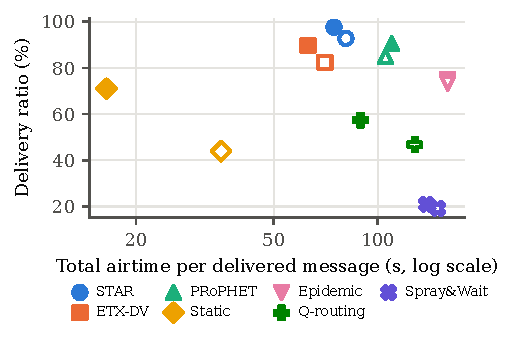
\includegraphics[width=\linewidth]{figures/pareto.pdf}
\caption{Delivery vs.\ total airtime per delivered message (log scale). Filled markers: baseline scenario; hollow markers: aftershock (20 seeds, means). STAR sits at the high-delivery end of the frontier at moderate cost.}
\label{fig:pareto}
\end{figure}

\subsection{Load}

\begin{figure*}[t]
\centering
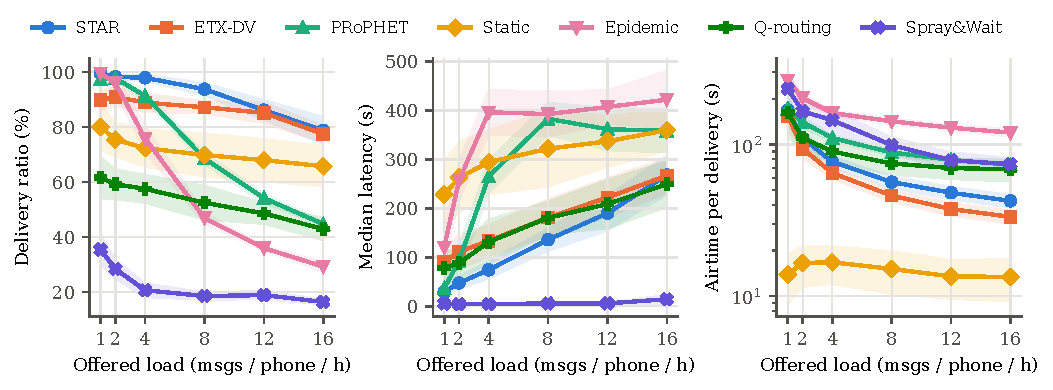
\includegraphics[width=\textwidth]{figures/load.pdf}
\caption{Load sweep (10 seeds per point; bands are 95\% CIs). STAR leads up to 8 messages per phone per hour; at saturation (12--16) its delivery converges with ETX-DV, while the replication protocols collapse as copies exhaust LoRa airtime.}
\label{fig:load}
\end{figure*}

Figure~\ref{fig:load} shows the regime in which learning helps. At low load STAR delivered 99.5\% with a 29\,s median latency. Its advantage over ETX-DV narrowed with load and disappeared at 12--16 messages per phone per hour (86.1\% vs.\ 85.2\% and 78.8\% vs.\ 77.5\%), where the LoRa channel, not route choice, limits throughput. Epidemic and PRoPHET, which match STAR at the lowest load, fell to 29\% and 45\% at the highest load as replicas consumed the channel.

\subsection{Aftershock}

\begin{table*}[t]
\centering
\caption{Aftershock scenario: at mid-run the microwave backbone and 30\% of shelter LoRa links fail permanently and one shelter crashes for 10\,min (20 seeds).}
\label{tab:aftershock}
\small
\resizebox{\textwidth}{!}{%
\begin{tabular}{lrrrrrr}
\toprule
Router & PDR (\%) & Confirmed (\%) & SOS PDR (\%) & Median lat.\ (s) & P95 lat.\ (s) & Airtime/deliv.\ (s) \\
\midrule
\textbf{STAR} & \textbf{92.8 $\pm$ 2.3} & \textbf{87.9 $\pm$ 2.9} & 95.1 $\pm$ 3.6 & 97 $\pm$ 18 & 634 $\pm$ 52 & 80.9 $\pm$ 4.0 \\
ETX-DV & 82.5 $\pm$ 2.5 & 71.5 $\pm$ 3.5 & 91.0 $\pm$ 4.4 & 172 $\pm$ 26 & 744 $\pm$ 29 & 70.4 $\pm$ 4.4 \\
PRoPHET & 84.9 $\pm$ 3.0 & 79.7 $\pm$ 4.3 & \textbf{97.1 $\pm$ 3.2} & 242 $\pm$ 29 & 766 $\pm$ 40 & 105.3 $\pm$ 3.8 \\
Static & 43.9 $\pm$ 3.8 & 39.2 $\pm$ 3.4 & 59.6 $\pm$ 11.5 & 199 $\pm$ 39 & 786 $\pm$ 45 & \textbf{35.2 $\pm$ 10.4} \\
Epidemic & 73.4 $\pm$ 3.2 & 62.4 $\pm$ 4.2 & 96.0 $\pm$ 3.1 & 410 $\pm$ 33 & 864 $\pm$ 19 & 159.4 $\pm$ 4.3 \\
Q-routing & 46.8 $\pm$ 2.6 & 27.7 $\pm$ 3.3 & 77.8 $\pm$ 5.7 & 170 $\pm$ 41 & 792 $\pm$ 41 & 128.0 $\pm$ 10.4 \\
Spray\&Wait & 19.1 $\pm$ 1.6 & 15.1 $\pm$ 1.3 & 46.2 $\pm$ 7.4 & \textbf{6 $\pm$ 2} & \textbf{463 $\pm$ 120} & 149.2 $\pm$ 15.6 \\
\bottomrule
\end{tabular}}
\end{table*}


\begin{figure}[t]
\centering
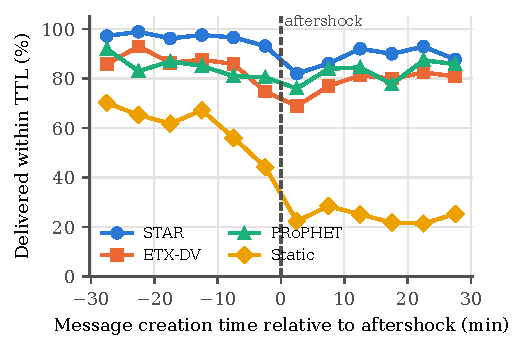
\includegraphics[width=\linewidth]{figures/aftershock.pdf}
\caption{Delivery ratio by message creation time around the aftershock (20 seeds pooled, 5-minute bins).}
\label{fig:aftershock}
\end{figure}

When the fast backbone and 30\% of shelter links disappeared, STAR kept the highest PDR (92.8\%, Table~\ref{tab:aftershock}), 10.3 points above ETX-DV ($p<10^{-7}$) and 7.8 above PRoPHET ($p<10^{-5}$). Static collapsed to 43.9\% because its preloaded routes kept pointing at dead links. Figure~\ref{fig:aftershock} shows the dynamics: every protocol loses messages created just before the event, whose routes vanish mid-flight; STAR recovers within one to two bins as its availability posteriors and feasible distances adapt. PRoPHET delivered slightly more SOS messages after the aftershock (97.1\% vs.\ 95.1\%; the intervals overlap) because it replicates everything.

\subsection{Route poisoning}

\begin{figure}[t]
\centering
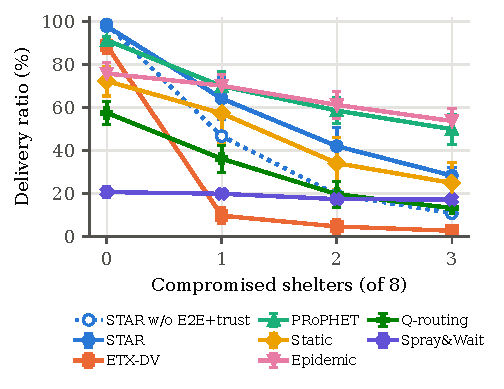
\includegraphics[width=\linewidth]{figures/blackhole.pdf}
\caption{Delivery under blackhole shelters that advertise perfect routes and drop traffic (10 seeds; error bars are 95\% CIs). The dotted line is STAR without end-to-end learning, trust, or watchdog.}
\label{fig:blackhole}
\end{figure}

A blackhole that advertises perfect routes captured almost all traffic of the unprotected ETX-DV protocol: its PDR fell from 88.9\% to 9.7\% with one compromised shelter (Figure~\ref{fig:blackhole}). STAR retained 64.2\%, 42.0\%, and 28.3\% with one, two, and three compromised shelters, against 46.7\%, 19.5\%, and 10.8\% for STAR without outcome learning; removing only the watchdog gave 51.0\%, 23.2\%, and 14.4\%. These defenses do not make single-copy routing as robust as replication: PRoPHET and Epidemic retained 50--70\%. Part of the gap is structural. With two compromised shelters, only about 70\% of messages in our topologies have any attacker-free path, because some phones attach only to a compromised shelter. The remainder reflects the learning delay before trust falls below the exclusion threshold.

\subsection{Ablation}

\begin{table*}[t]
\centering
\caption{Ablation of STAR components (20 evaluation seeds, mean $\pm$ 95\% CI). PDR = packet delivery ratio.}
\label{tab:ablation}
\small
\resizebox{\textwidth}{!}{%
\begin{tabular}{llrrrrrr}
\toprule
 & & \multicolumn{3}{c}{Baseline scenario} & \multicolumn{3}{c}{Aftershock scenario} \\
\cmidrule(lr){3-5}\cmidrule(lr){6-8}
Variant & Removed component & PDR (\%) & SOS (\%) & Med.\ lat.\ (s) & PDR (\%) & SOS (\%) & Med.\ lat.\ (s) \\
\midrule
\textbf{STAR} & Full model & 97.7 $\pm$ 0.9 & 100.0 $\pm$ 0.0 & 74 $\pm$ 11 & 92.8 $\pm$ 2.3 & 95.1 $\pm$ 3.6 & 97 $\pm$ 18 \\
STAR-noTS & no Thompson sampling (posterior means) & 97.8 $\pm$ 0.7 & 99.2 $\pm$ 1.1 & 80 $\pm$ 11 & 92.5 $\pm$ 2.6 & 97.9 $\pm$ 1.7 & 108 $\pm$ 23 \\
STAR-noRisk & no risk-averse LCB for P0/P1 & 97.6 $\pm$ 0.9 & 100.0 $\pm$ 0.0 & 74 $\pm$ 10 & 92.4 $\pm$ 2.1 & 95.9 $\pm$ 3.6 & 99 $\pm$ 18 \\
STAR-noStab & no stability score ($\Psi$ $\to$ min.\ delay) & 95.4 $\pm$ 1.5 & 99.2 $\pm$ 1.1 & 63 $\pm$ 10 & 88.6 $\pm$ 2.9 & 97.2 $\pm$ 2.8 & 78 $\pm$ 13 \\
STAR-noE2E & no end-to-end learning or trust & 98.2 $\pm$ 1.0 & 99.5 $\pm$ 1.0 & 64 $\pm$ 11 & 92.5 $\pm$ 2.6 & 98.7 $\pm$ 1.9 & 85 $\pm$ 19 \\
STAR-noWatch & no watchdog overhearing & 98.3 $\pm$ 0.7 & 100.0 $\pm$ 0.0 & 65 $\pm$ 10 & 92.8 $\pm$ 2.6 & 97.9 $\pm$ 2.2 & 93 $\pm$ 18 \\
STAR-noSpray & no SOS replication & 98.1 $\pm$ 0.8 & 100.0 $\pm$ 0.0 & 72 $\pm$ 11 & 92.5 $\pm$ 2.1 & 95.4 $\pm$ 3.6 & 102 $\pm$ 20 \\
STAR-noDecay & no posterior discounting & 98.3 $\pm$ 0.6 & 100.0 $\pm$ 0.0 & 69 $\pm$ 9 & 92.5 $\pm$ 2.5 & 98.8 $\pm$ 1.8 & 93 $\pm$ 15 \\
\bottomrule
\end{tabular}}
\end{table*}


Table~\ref{tab:ablation} isolates the components. The stability score is the component with the largest and only statistically significant effect: replacing $\Psi$ by minimum expected delay lowered PDR by 2.3 points in the baseline scenario ($p=0.002$) and by 4.2 points after the aftershock ($p<10^{-4}$), while reducing median latency by 11--19\,s. This is the expected trade-off: stability-aware choice accepts slightly longer routes that are less likely to fail. The other components had no detectable effect on delivery in attack-free scenarios. Thompson sampling, discounting, SOS replication, the watchdog, and end-to-end learning changed PDR by less than 1 point (all $p>0.1$), and the security mechanisms cost about 9--12\,s of median latency because their conservative trust estimates occasionally steer traffic away from honest neighbors. Their value appears under attack (Figure~\ref{fig:blackhole}) and, for discounting and exploration, in non-stationary conditions that our 1-hour scenarios exercise only partly. We report these null results because they bound what the full model should be credited with.

\subsection{Prediction quality}

\begin{figure*}[t]
\centering
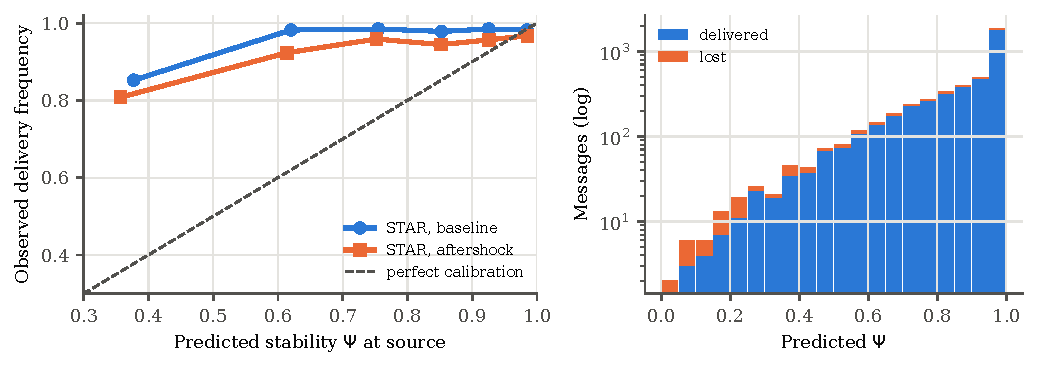
\includegraphics[width=0.85\textwidth]{figures/calibration.pdf}
\caption{Left: reliability of the raw stability score $\Psi$ at the source (bins with at least 10 messages). Right: distribution of $\Psi$ for delivered and lost messages (log scale).}
\label{fig:calibration}
\end{figure*}

The raw score is informative but conservative (Figure~\ref{fig:calibration}). Over 4{,}408 source decisions it separated delivered from lost messages with AUC 0.69, but its mean (0.85) was below the observed delivery rate (0.96), so its Brier score (0.069) was worse than a constant forecast at the base rate (0.038). The bias has a clear cause: $\Psi$ evaluates a \emph{fixed} route, whereas downstream nodes re-route adaptively, and messages that miss one opportunity usually find another. $\Psi$ therefore behaves as a lower bound, which is the safe direction for a quantity that triggers SOS replication. Because the bias is monotone, a two-parameter logistic recalibration learned from receipt outcomes fixes it: fitted on seeds 100--109 and tested on 110--119, the recalibrated score had a Brier score of 0.038 against 0.040 for the base-rate forecast, with predicted and observed frequencies within 1--2 points in the bins that hold 97\% of messages. Ranking, which drives routing, is unaffected by such recalibration; reported delivery probabilities, for example in a user interface, should use the recalibrated value.

\section{Discussion}

\textbf{What the model learns.} STAR's gains come from two sources. First, availability posteriors with silence-aware decay let a node distinguish a lossy-but-present link from an absent one and hold traffic rather than retransmit into a dead link, which matters on LoRa, where a failed exchange can waste seconds of channel time. Second, the stability score prefers routes whose delay is both short and predictable relative to the remaining lifetime. Shortest-delay routing gets the first benefit but not the second, which explains the ablation.

\textbf{When not to expect gains.} At saturation, delivery is bounded by channel capacity, and STAR's slightly larger control entries and longer routes cost about as much as better route choice gains. On single paths there is nothing to choose. Against insiders, single-copy custody is fundamentally exposed while trust is being learned; a deployment could replicate SOS messages unconditionally during the first minutes after a topology change.

\textbf{Privacy.} Advertisements expose which mailboxes are reachable through which neighbors. TRCN's rotating pairwise mailboxes limit linkage across epochs, but routing summaries remain metadata that a passive observer can collect; aggregating destinations by region would reduce exposure at the cost of precision.

\textbf{Safety.} STAR never reports delivery itself. Only signed receipts do, consistent with TRCN's rule that the user interface must never show a false success. Predicted probabilities shown to users should be recalibrated, and phrased as estimates.

\textbf{Threats to validity.} All results are synthetic. The link process is exponential on/off with Bernoulli frame loss, whereas real outages are often heavy-tailed and spatially correlated. Collision domains are region-wide with no capture effect, hidden terminals, or half-duplex constraints. Duty-cycle limits and Taiwanese low-power radio regulations \parencite{ncclp0002} are not modeled, phones do not move between shelters, and the blackhole attacker is not adaptive (it does not, for example, forward only overheard traffic). Parameters were tuned on development seeds of the same generator, so results on other topologies may differ. Each of these is a direction for field measurement, not a claim of the paper.

\section{Conclusion}

STAR shows that a node can predict, using only what it observes, which neighbor is most likely to deliver a message on time, and can improve that prediction from the outcomes of its own decisions. Composing Bayesian link posteriors with loop-free, authenticated summaries into a deadline-aware stability score raised delivery and lowered latency against strong baselines in synthetic disaster networks, and outcome-calibrated trust kept route poisoning from capturing the network. The next steps are durable custody, real radios under legal operating conditions, and traces from communities that would use such a network.

\section*{Data and Code Availability}
The simulator (\texttt{trcn\_star/}), experiment scripts (\texttt{experiments/}), raw per-run results (\texttt{results/}), and unit tests (\texttt{tests/}) are available at \url{https://github.com/chengmatt416/trcn}. \texttt{python experiments/run\_all.py} followed by \texttt{python experiments/plots.py} regenerates every table and figure.

\section*{Use of Generative AI}
This research was conducted with substantial assistance from generative artificial intelligence. The initial TRCN design notes (protocol specification, threat model, benchmark notes, and roadmap) on which this work builds were produced with ChatGPT (OpenAI). Claude (Anthropic; model Claude Opus 5.5) was then used, under the author's direction, to (a) search the literature and check each reference against publisher, standards-body, DBLP, or arXiv records; (b) design the STAR model and implement the simulator, baselines, unit tests, and experiment scripts; (c) run the experiments and statistical analyses; and (d) draft and edit the manuscript, tables, and figures. All numerical results come from executing the released code, not from text generated by a model, and can be regenerated with the scripts listed under Data and Code Availability. The author, Pinyen Cheng, defined the research goal, reviewed the outputs, and takes full responsibility for the content of this article.

\printbibliography

\appendix
\section{Parameters}

\begin{table}[h]
\caption{STAR parameters (frozen before evaluation)}
\label{tab:params}
\small
\begin{tabularx}{\linewidth}{@{}lrY@{}}
\toprule
Symbol & Value & Meaning \\
\midrule
$B$ & 60\,s & beacon period (all adaptive routers) \\
$(\alpha_0,\beta_0)_f$ & (4, 1) & frame-success prior \\
$(\alpha_0,\beta_0)_u$ & (3, 1) & availability prior \\
$H_f$, $H_u$ & 900, 240\,s & posterior half-lives \\
$H_s$ & 600\,s & staleness half-life of claims \\
$H_e$ & 1200\,s & half-life of end-to-end counts \\
$K$ & 4 & pseudo-counts for a calibrated claim \\
$\tau_{\min}$ & 0.4 & trust exclusion threshold \\
$\varepsilon$, $\varepsilon_{P0}$ & 0.03, 0.01 & $\Psi$ tolerance for delay tie-break \\
$\Psi^\ast$, $L_{\max}$ & 0.95, 3 & SOS replication target and cap \\
$z$ & 1.28 & lower-bound quantile (10\%) for P0/P1 \\
--- & 24 & advertisement entries per beacon \\
--- & 4 & beacons per sequence-number increment \\
--- & 4 & rounds per exchange \\
\bottomrule
\end{tabularx}
\end{table}

\end{document}
